\documentclass[12pt,]{article}
\usepackage[utf8]{inputenc}
\usepackage[T1]{fontenc}
\usepackage{mathptmx}
\usepackage{geometry}
\usepackage{mathtools}
\usepackage[english]{babel}
\usepackage{graphicx}
\usepackage[os=win]{menukeys}
\usepackage[figurename=Gambar]{caption}
\usepackage{hyperref}
\usepackage{minted}
\usepackage{float}
\usepackage{pdflscape}
\usepackage{pdfpages}
\usepackage{tikz}

\addto\captionsenglish{\renewcommand{\contentsname}{Daftar Isi}}
\addto\captionsenglish{\renewcommand{\bibname}{Referensi}}

\geometry{
	legalpaper,
	left=15mm,
	right=10mm,
	top=10mm,
	bottom=10mm,
}

\usetikzlibrary{positioning}
\tikzstyle{squared} = [rectangle, rounded corners, minimum width=1cm, minimum height=0.5cm,text centered, draw=black]
\tikzstyle{connect} = [ultra thick,->]
\tikzstyle{connect2} = [ultra thick,<->]

\title{\Large \bf
	Pengenalan Pemrograman C dan chip seri ATMega.
}

\author{Achmadi ST MT}
\date{}

\begin{document}
	\maketitle
	\thispagestyle{empty}
	\pagestyle{empty}
	
	\newpage
	\tableofcontents
	
	\newpage
	\section{Requirement}
	
	Dalam pengembangan aplikasi berbasis ATMega, dibutuhkan beberapa hardware dan software.
	Berikut akan disebutkan dan dijelaskan untuk beberapa sistem operasi:
	
	\subsection{Software}
	
	\subsubsection{Code::Blocks}
	Code::Blocks adalah suatu program lingkungan pengembangan terpadu bebas, gratis, bersumber terbuka dan lintas platform.
	Program yang ditulis dalam C++ beserta wxWidgets untuk GUI-nya ini bisa digunakan bersama dengan berbagai macam kompilator, contohnya GCC dan CLang.
	Peralatannya yang tersedia tergantung dari "plugin" yang ada dipasang.
	Sekarang ini, Code::Blocks lebih tersedia sebagai perangkat pengembangan dalam bahasa C dan C++, walaupun program ini juga bisa disesuaikan, 
	dan mungkin akan membutuhkan pemasangan tambahan, untuk pengembangan perangkat lunak ARM, AVR, Fortran, GLFW, GLUT, GTK+,  MATLAB, OGRE, OpenGL, Qt, atau SDL.
	Code::Blocks tersedia di sistem operasi Windows, Linux, Mac OS X dan FreeBSD.
	\begin{figure}[H]
		\centering
		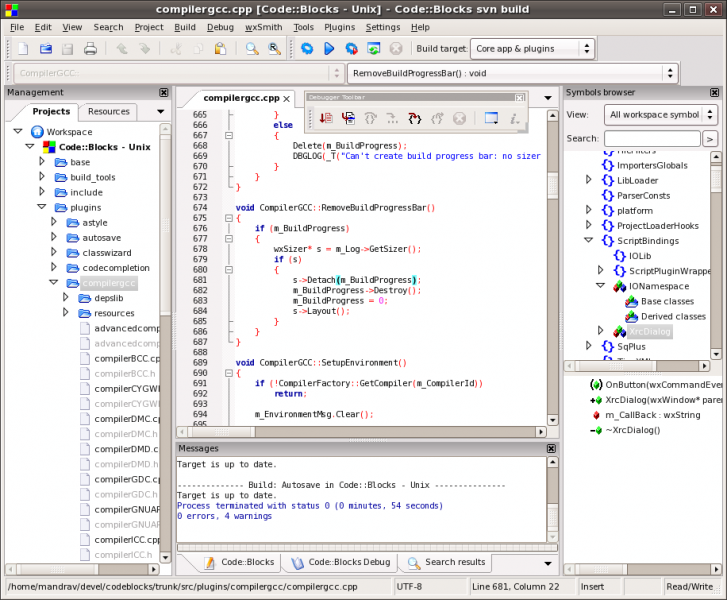
\includegraphics[width=0.6\linewidth]{images/cb}
		\caption{contoh tampilan Code::Blocks}
	\end{figure}

	Berikut instalasi:
	\begin{itemize}
		\item Windows.
		\begin{itemize}
			\item Buka alamat \url{http://www.codeblocks.org/downloads/26}.
			\item Klik file codeblocks-17.12mingw-setup.exe.
			\item Tunggu proses download selesai.
			\item Jalankan file codeblocks-17.12mingw-setup.exe untuk instalasi.
		\end{itemize}
	
		\item Ubuntu/Debian.
		\begin{itemize}
			\item Buka Terminal (pastikan terhubung internet).
			\item Masukkan perintah.
				\begin{minted}[frame=lines,fontsize=\footnotesize]{bash}
sudo apt-get install codeblocks build-essential
				\end{minted}
			\item Tunggu proses selesai.
		\end{itemize}
	
		\item Fedora.
		\begin{itemize}
			\item Buka Terminal (pastikan terhubung internet).
			\item Masukkan perintah.
				\begin{minted}[frame=lines,fontsize=\footnotesize]{bash}
sudo dnf groupinstall 'Development Tools'
sudo dnf install codeblocks
				\end{minted}
			\item Tunggu proses selesai.
		\end{itemize}
	
		\item Arch-Linux.
		\begin{itemize}
			\item Buka Terminal (pastikan terhubung internet).
			\item Masukkan perintah.
			\begin{minted}[frame=lines,fontsize=\footnotesize]{bash}
sudo pacman -S codeblocks base-devel 
			\end{minted}
			\item Tunggu proses selesai.
		\end{itemize}

	\end{itemize}

	\subsubsection{GCC AVR}
	GCC adalah software kompilasi gratis dan bebas untuk chip AVR.
	GCC (GNU C Compiler) bertugas mengkompilasi kode sumber menjadi file \textit{binary} yang siap dijalankan atau di-\textit{download} ke dalam chip.

	Berikut instalasi:
	\begin{itemize}
		\item Windows.
		\begin{itemize}
			\item Download file instalasi di alamat:
			\begin{itemize}
				\item Windows x86 (32bit): \url{http://blog.zakkemble.net/download/avr-gcc-8.3.0-x86-mingw.zip}
				\item Windows x64 (64bit): \url{http://blog.zakkemble.net/download/avr-gcc-8.3.0-x64-mingw.zip}
			\end{itemize}
			\item Extrak file yang sudah di download.
			\item Masukkan alamat kompiler dalam \textit{binary path} milik Windows.
		\end{itemize}
	
		\item Ubuntu/Debian.
		\begin{itemize}
			\item Buka Terminal (pastikan terhubung internet).
			\item Masukkan perintah.
			\begin{minted}[frame=lines,fontsize=\footnotesize]{bash}
sudo apt-get install gcc-avr binutils-avr avr-libc
			\end{minted}
			\item Tunggu proses selesai.
		\end{itemize}
		
		\item Fedora.
		\begin{itemize}
			\item Buka Terminal (pastikan terhubung internet).
			\item Masukkan perintah.
			\begin{minted}[frame=lines,fontsize=\footnotesize]{bash}
sudo dnf install avr-binutils avr-gcc avr-libc
			\end{minted}
			\item Tunggu proses selesai.
		\end{itemize}
		
		\item Arch-Linux.
		\begin{itemize}
			\item Buka Terminal (pastikan terhubung internet).
			\item Masukkan perintah.
			\begin{minted}[frame=lines,fontsize=\footnotesize]{bash}
sudo pacman -S avr-binutils avr-gcc avr-lib 
			\end{minted}
			\item Tunggu proses selesai.
		\end{itemize}
			
	\end{itemize}

	\subsubsection{Downloader}
	Download adalah software bantu untuk download (memasukkan) binary hasil kompilasi ke dalam chip.
	Tersedia banyak software tergantung tipe hardware downloader yang dipakai.
	Untuk kursus ini, digunakan downloader berbasis UASAsp, maka software downloader yang digunakan adalah
	Khazama untuk Windows dan avrdude (AVR Downloader/UploaDEr) untuk selain Windows.
	
	Berikut instalasi:
	\begin{itemize}
		\item Windows
		\begin{figure}[H]
			\centering
			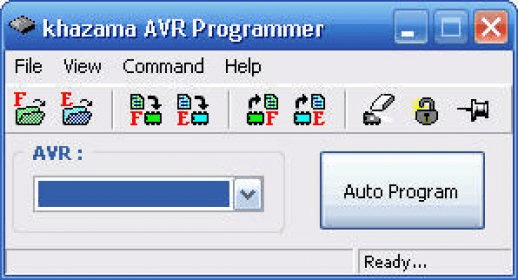
\includegraphics[width=0.4\linewidth]{images/khazama}
			\caption{contoh tampilan Khazama}
		\end{figure}
		\begin{itemize}
			\item Download file instalasi Khazama 1.6 di alamat \url{http://khazama.com/project/programmer/KhazamaAVRProgrammer162.rar}.
			\item Ekstrak file yang di download dan jalankan file installernya.
		\end{itemize}
	
		\item Ubuntu/Debian.
		\begin{itemize}
			\item Buka Terminal (pastikan terhubung internet).
			\item Masukkan perintah.
			\begin{minted}[frame=lines,fontsize=\footnotesize]{bash}
sudo apt-get install avrdude
			\end{minted}
			\item Tunggu proses selesai.
		\end{itemize}
		
		\item Fedora.
		\begin{itemize}
			\item Buka Terminal (pastikan terhubung internet).
			\item Masukkan perintah.
			\begin{minted}[frame=lines,fontsize=\footnotesize]{bash}
sudo dnf install avrdude
			\end{minted}
			\item Tunggu proses selesai.
		\end{itemize}
		
		\item Arch-Linux.
		\begin{itemize}
			\item Buka Terminal (pastikan terhubung internet).
			\item Masukkan perintah.
			\begin{minted}[frame=lines,fontsize=\footnotesize]{bash}
sudo pacman -S avrdude
			\end{minted}
			\item Tunggu proses selesai.
		\end{itemize}

	\end{itemize}

	\subsubsection{Simul-IDE}
	
	Dalam kursus ini, untuk awal pelatihan, digunakan Simulator untuk menjalankan dan menguji program AVR yang dibuat.
	Simulator yang dipilih disini adalah Simul-IDE. 
	Simul-IDE adalah simulator rangkaian elektronik Digital/Analog sederhana yang dapat berjalan secara \textit{real-time}.
	Simul-IDE dapat mendukung microcontroller seperti chip seri AVR ataupun PIC.
	
	\begin{figure}[H]
		\centering
		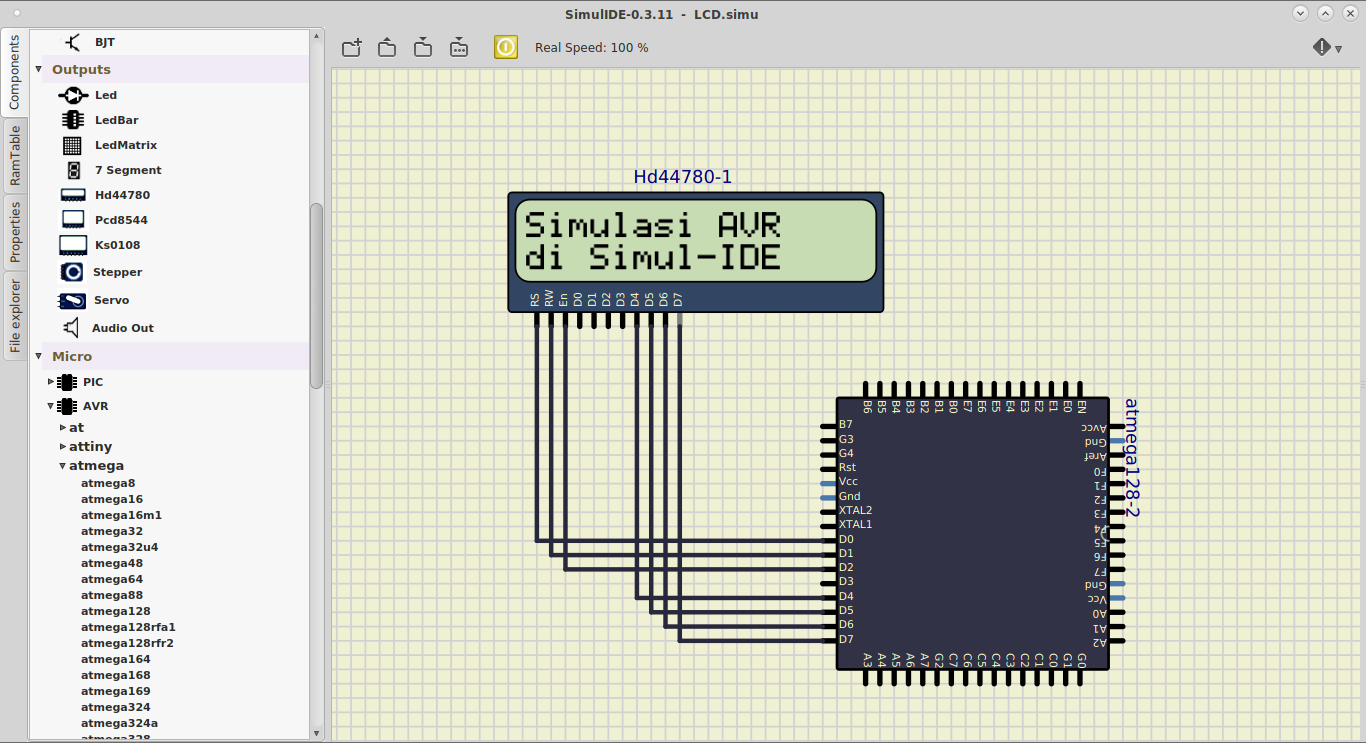
\includegraphics[width=0.6\linewidth]{images/simul}
		\caption{contoh tampilan Simul-IDE}
	\end{figure}

	Berikut untuk instalasi:
	\begin{itemize}
		\item Windows
		\begin{itemize}
			\item Buka alamat \url{https://sourceforge.net/projects/simulide/files/SimulIDE_0.3.10/SimulIDE_0.3.10_SR1-Win32.zip/download}
			\item Ekstrak file yang sudah di download.
			\item Jalankan file \textbf{run\_simulide.bat}.
		\end{itemize}
	
		\item Ubuntu/Debian.
		\begin{itemize}
			\item Buka Terminal (pastikan terhubung internet).
			\item Masukkan perintah.
			\begin{minted}[frame=lines,fontsize=\footnotesize]{bash}
sudo apt-get install simulide simavr
			\end{minted}
			\item Tunggu proses selesai.
			\item Buka terminal dimana project AVR berada.
			\item Masukkan perintah:
			\begin{minted}[frame=lines,fontsize=\footnotesize]{bash}
simulide
			\end{minted}
		\end{itemize}
	
		\item Fedora.
		\begin{itemize}
			\item Buka Terminal (pastikan terhubung internet).
			\item Masukkan perintah.
			\begin{minted}[frame=lines,fontsize=\footnotesize]{bash}
sudo dnf install simulide simavr
			\end{minted}
			\item Tunggu proses selesai.
			\item Buka terminal dimana project AVR berada.
			\item Masukkan perintah:
			\begin{minted}[frame=lines,fontsize=\footnotesize]{bash}
simulide
			\end{minted}
		\end{itemize}
	
		\item Arch Linux.
		\begin{itemize}
			\item Buka Terminal (pastikan terhubung internet).
			\item Masukkan perintah.
			\begin{minted}[frame=lines,fontsize=\footnotesize]{bash}
sudo pacman -S simavr
			\end{minted}
			\item Tunggu proses selesai.
			\item Download resep AUR di \url{https://aur.archlinux.org/cgit/aur.git/snapshot/simulide.tar.gz}
			\item Ekstrak file tersebut dan buka terminal di alamat tersebut.
			\item Masukkan perintah:
			\begin{minted}[frame=lines,fontsize=\footnotesize]{bash}
makepkg -sir
			\end{minted}
			\item Tunggu proses instalasi selesai
			\item Buka terminal dimana project AVR berada.
			\item Masukkan perintah:
			\begin{minted}[frame=lines,fontsize=\footnotesize]{bash}
simulide
			\end{minted}
		\end{itemize}
		
	\end{itemize}

	\subsubsection{KiCad}
	KiCad adalah software bebas dan gratis untuk membantu merancang circuit elektronik.
	KiCad menyediakan fitur olah skematik, layout PCB, dan 3D visualisasi.
	
	\begin{figure}[H]
		\centering
		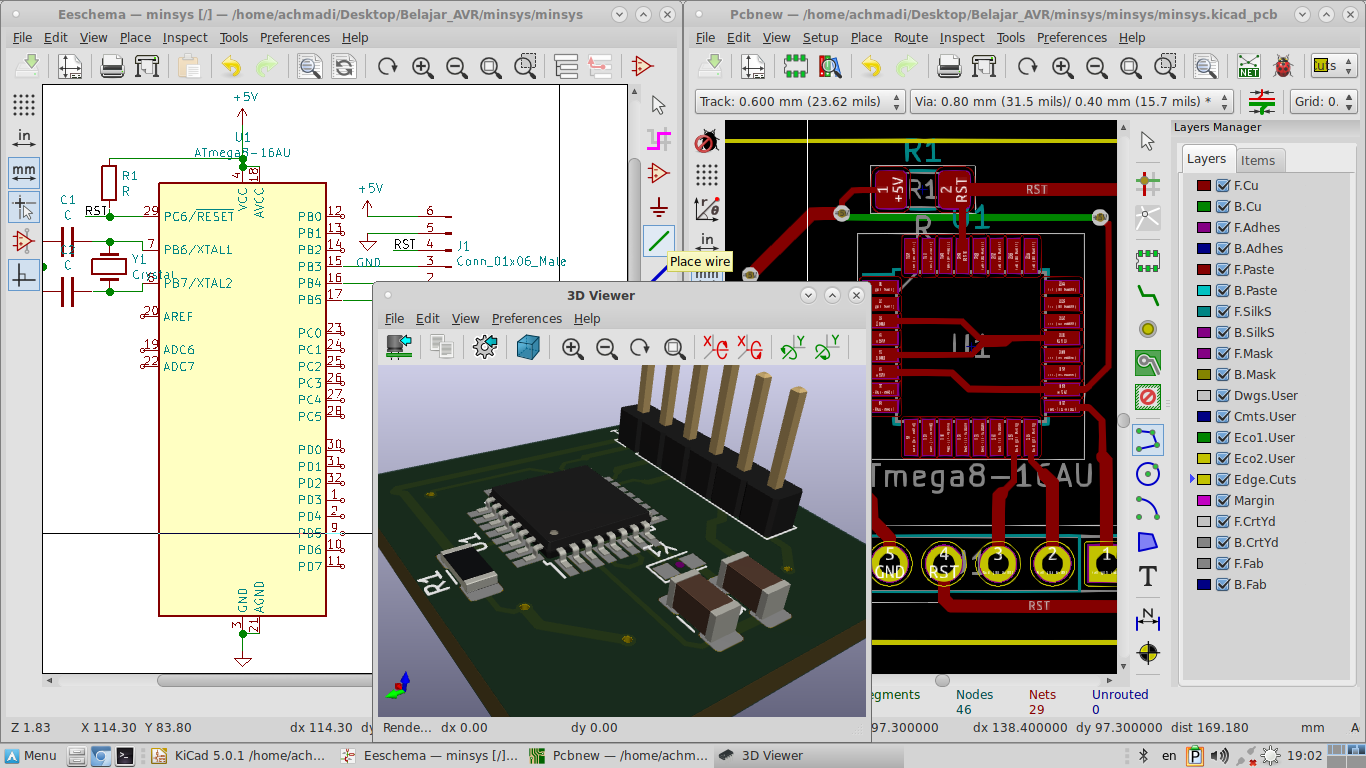
\includegraphics[width=0.6\linewidth]{images/kicad}
		\caption{contoh tampilan KiCAD}.
	\end{figure}

	Berikut untuk instalasi:
	\begin{itemize}
		\item Windows
		\begin{itemize}
			\item Buka alamat \url{http://kicad-pcb.org/download/windows/}
			\item Pilih dan download file instalasi sesuai laptop/komputer anda.
			\item Jalankan file instalasi.
		\end{itemize}
	
		\item Ubuntu/Debian.
		\begin{itemize}
			\item Buka Terminal (pastikan terhubung internet).
			\item Masukkan perintah.
			\begin{minted}[frame=lines,fontsize=\footnotesize]{bash}
sudo add-apt-repository ppa:js-reynaud/kicad-5
sudo apt-get update
sudo apt-get install kicad
			\end{minted}
			\item Tunggu proses selesai.
		\end{itemize}
		
		\item Fedora.
		\begin{itemize}
			\item Buka Terminal (pastikan terhubung internet).
			\item Masukkan perintah.
			\begin{minted}[frame=lines,fontsize=\footnotesize]{bash}
sudo dnf install kicad kicad-packages3d
			\end{minted}
			\item Tunggu proses selesai.
		\end{itemize}
		
		\item Arch Linux.
		\begin{itemize}
			\item Buka Terminal (pastikan terhubung internet).
			\item Masukkan perintah.
			\begin{minted}[frame=lines,fontsize=\footnotesize]{bash}
sudo pacman -S kicad kicad-library kicad-library-3d
			\end{minted}
			\item Tunggu proses selesai.
		\end{itemize}
		
	\end{itemize}

	\subsection{Hardware}
	
	Untuk hardware, kebutuhan pokok dalam membangun aplikasi ATMega hanyalah 2 saja, yaitu: Downloader dan Minimum-System 
	
	\subsubsection{Downloader}
	Downloader adalah hardware yang digunakan untuk memasukkan program dalam chip.
	Tipe downloader yang digunakan disini adalah USBAsp dimana baik skematik maupun firmware yang digunakan bersifat open-source.
	USBAsp secara mendasar hanya membutuhkan:
	\begin{itemize}
		\item ATMega48, ATMega8, atau ATMega88
		\item Clock 12MHz atau lebih
		\item 2 PIN untuk jalur VCC dan GND
		\item 4 PIN untuk jalur SPI (SS, MOSI, MISO, dan SCK)
		\item 4 PIN untuk jalur USB (VCC, GND, D+, dan D-)
	\end{itemize}
	Project USBAsp dapat anda temukan di alamat \url{https://www.fischl.de/usbasp/}.
	Sedangkan untuk hardware dapat anda beli di pasaran dengan harga terjangkau atau anda dapat merakit sendiri.
	\begin{figure}[H]
		\centering
		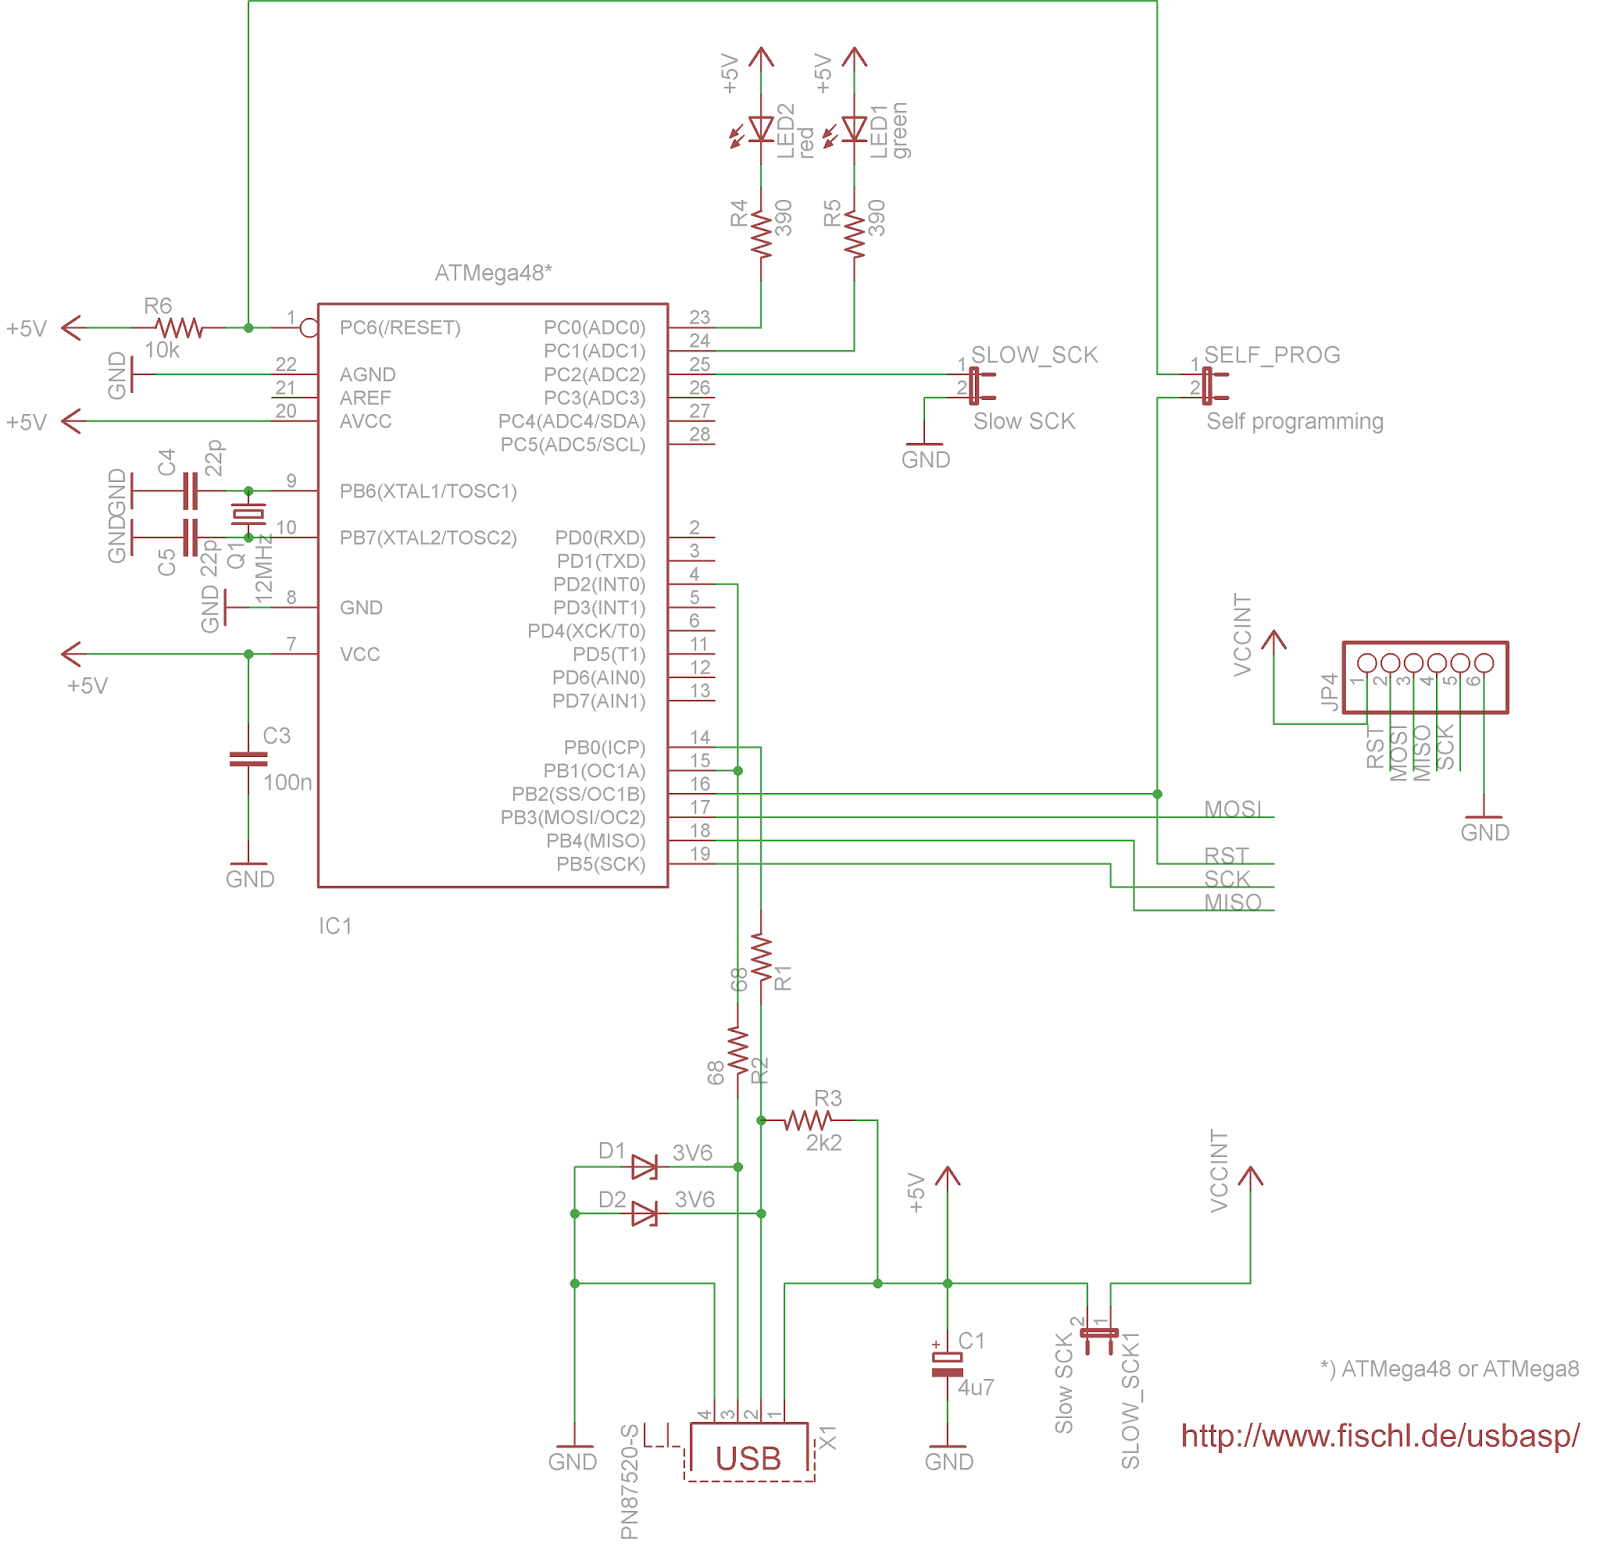
\includegraphics[width=0.6\linewidth]{images/usbasp}
		\caption{contoh skematik USBAsp}
	\end{figure}

	\textbf{Advance}: Selain menggunakan USBAsp fisik, anda dapat juga menanamkan \textit{virtual} downloader USBAsp kedalam bagian \textit{bootloader} ATMega.
	Keuntungannya anda tidak lagi perlu USBAsp fisik terpisah dengan Minimum-System,
	namun kekurangannya adalah alamat aplikasi berpindah ke alamat bootloader sehingga terkadang memory tidak sampai alamat aplikasi.
	Project ini dikenal dengan USBAspLoader dan dapat anda temukan di \url{https://www.obdev.at/products/vusb/usbasploader.html}.
	
	\subsubsection{Minimum-System}
	Minimum-System didefiniskan sebagai rangkaian dasar agar chip ATMega dapat berjalan.
	Pada dasarnya ATMega hanya membutuhkan:
	\begin{itemize}
		\item Power VCC (5v) dan GND (0v). Power ini bisa didapat dari tegangan USB atau output regulator 7805/LM2569s.
		\item 5 PIN untuk download via SPI (GND, RST, MOSI, MISO, dan SCK) jika ingin didownload \textit{on-board}.
		\item Crystal (XTALL) atau RTC jika sumber Clock ATMega di set eksternal.
	\end{itemize}

	\begin{figure}[H]
		\centering
		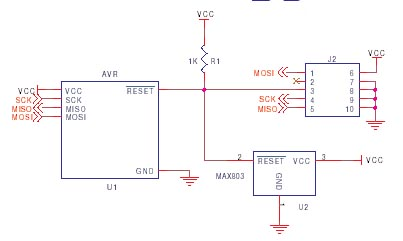
\includegraphics[width=0.6\linewidth]{images/minsys}
		\caption{contoh diagram dasar Minimum-System}
	\end{figure}

	\section{Bahasa C}
	
	
	
\end{document}